% common arguments
\newcommand{\coursenum}[0]{CSCI 0452}%
\newcommand{\coursetitletop}[0]{Image}%
\newcommand{\coursetitlebottom}[0]{Processing}%
\newcommand{\bordercolor}[0]{7905FA}%
\newcommand{\backgroundcolor}[0]{white}%


\documentclass{standalone}
\usepackage{graphicx}
\usepackage{tikz}
\usepackage{xcolor}
\usepackage{inconsolata} % change to control font
\renewcommand*\familydefault{\ttdefault} 
\usepackage[T1]{fontenc}

\begin{document}

\definecolor{border_color}{HTML}{\bordercolor}%

\begin{tikzpicture}

  \newdimen\R
  \R=1in

  \node[]             at   (0.1, 0)     {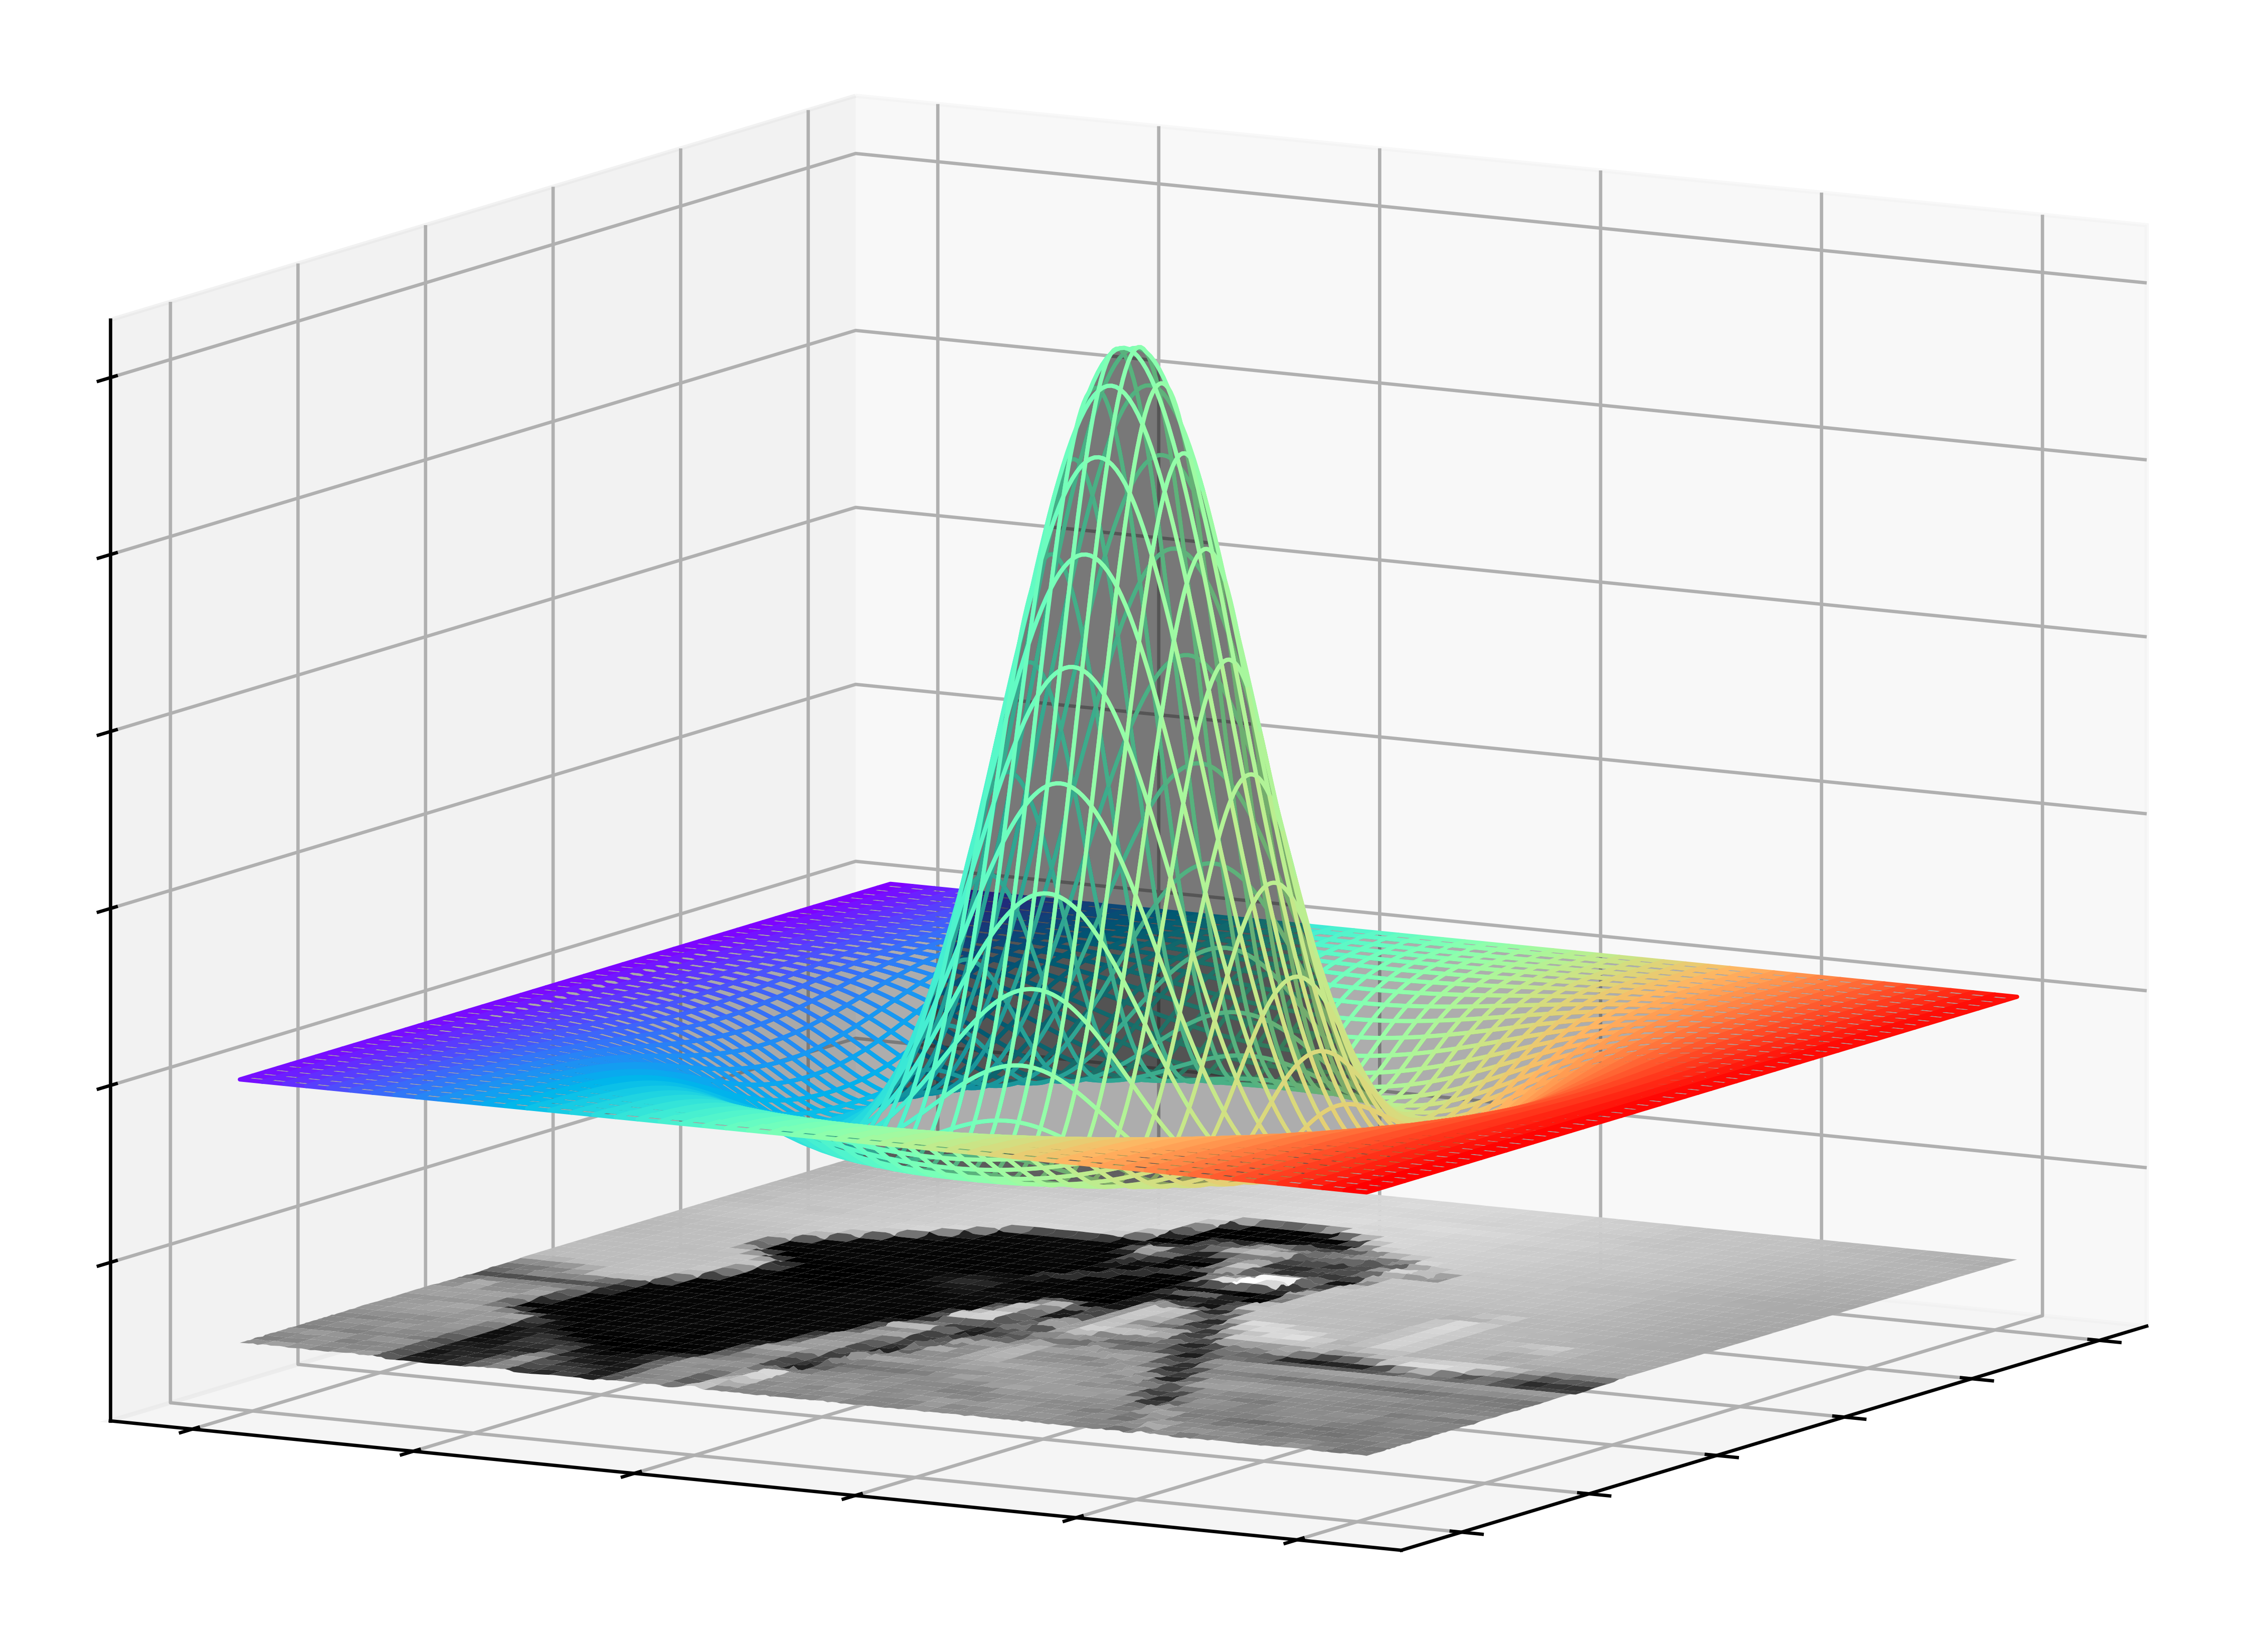
\includegraphics[height=0.8 in]{laplacian.png}};
  \node[align=center] at  (90:0.52in) {\Large \ttfamily \bfseries \coursenum};
  \node[align=center] at (270: 0.55 in) {\large \ttfamily \coursetitletop \\ \large \ttfamily \coursetitlebottom};
  
  \draw[rounded corners=0.3mm,line width=1.3mm,color=border_color]
    (30:\R)--(90:\R)--(150:\R)--(210:\R)--(270:\R)--(330:\R)--cycle;

  \end{tikzpicture}

\end{document}


